\documentclass[12pt,a4paper]{article}
\usepackage[utf8]{inputenc}
\usepackage[ukrainian]{babel}
\usepackage{amsmath}
\usepackage{amsfonts}
\usepackage{amssymb}
\usepackage{graphicx}
\usepackage{hyperref}
\usepackage[left=2cm,right=2cm,top=2cm,bottom=2cm]{geometry}

% Define custom command for text reference
\newcommand{\textref}[2]{\hyperref[#1]{#2}}

\begin{document}

\begin{titlepage}
    \centering
    \vspace*{1cm}

    \Large
    Київський національний університет імені Тараса Шевченка \\

    \vspace{0.5cm}

    \large
    Факультет комп'ютерних наук та кібернетики \\

    \vspace{0.5cm}

    Кафедра інтелектуальних інформаційних систем \\

    \vspace{0.5cm}

    Алгебро-автоматичні методи проектування програмного забезпечення \\

    \vspace{3cm}

    \textbf{Лабораторна робота 3} \\

    \vspace{0.5cm}

    Скінченні автомати \\
    Композиція автоматів Б'юхі. \\

    \vspace{2cm}

    Виконали студенти 1-го курсу \\

    \vspace{0.2cm}

    Групи ПЗС-1 \\

    \vspace{0.1cm}

    Рябов Кирило \\

    \vspace{0.1cm}

    Соколов Михайло \\

    \vspace{0.1cm}

    Рибачок Руслан \\

    \vfill

    2023

\end{titlepage}

\section*{Лабораторна 3: Композиція автоматів Б'юхі. }

\textbf{Мета:} розгляд процесу композиції двох автоматів Б'юхі

\subsection*{Посилання на репозиторій з кодом:}

\href{https://github.com/KyrylR/Automata-1-2023-labs}{https://github.com/KyrylR/Automata-1-2023-labs}

\subsection*{Псевдокод:}

\begin{flalign*}
& \textbf{Вхід:} \quad \text{Регулярні w-мови } L \text{ і } L1. \\
& \textbf{Вихід:} \quad \text{Автомат } B \text{, який акцептує конкатенацію } L \cdot L1. \\
& \textbf{Метод:} &
\end{flalign*}

\begin{enumerate}
    \item Користуючись алгоритмами синтезу скінченних автоматів, побудуємо автомати \( A \) та \( A1 \), які акцептують мови \( L \) та \( L1 \) відповідно.

    \item Побудуємо відповідні двополюсники \( B \) та \( C \) для автоматів \( A \) та \( A1 \) відповідно.

    \item Побудуємо w-автомат \( C' \), застосувавши операцію сильної ітерації до \( C \).

    \item Побудуємо конкатенацію автоматів \( B \) та \( C' \), використовуючи операцію конкатенації автоматів. Це включає в себе наступні кроки:
    \begin{enumerate}
        \item Створимо новий автомат зі станами у вигляді декартового добутку станів \( B \) та \( C' \).

        \item Визначимо функцію переходу, базуючись на переходах \( B \) та \( C' \).

        \item Встановимо початковий стан як кортеж початкових станів \( B \) та \( C' \).

        \item Визначимо приймаючі стани як приймаючі стани \( C' \).
    \end{enumerate}

    \item Повернемо результати автомату \( B \), який акцептує конкатенацію мов \( L \) та \( L1 \).
\end{enumerate}

\section*{Пояснення}

Наданий алгоритм призначений для композиції двох автоматів Б'юхі в один автомат Б'юхі. Він слідує систематичному процесу об'єднання станів, алфавітів, переходів, початкових станів та приймаючих станів двох вхідних автоматів для формування складеного автомата.  \\

\setlength{\parindent}{0pt}Перший крок алгоритму конкатенації, який полягає у побудові автоматів \(A\) та \(A1\) для прийняття мов \(L\) та \(L1\), було вже виконано в співпраці з підгрупою 6. Таким чином, в нашому звіті використовуються вже синтезовані скінченні автомати, і ми пропускаємо демонстрацію процесу побудови регулярних виразів для цих мов, переходячи відразу до наступних кроків алгоритму. \\

\setlength{\parindent}{0pt}Основні кроки алгоритму можна підсумувати наступним чином:

\begin{enumerate}
    \item \textbf{Композиція станів}:
    \begin{itemize}
        \item Алгоритм формує набір станів для складеного автомата, обчислюючи декартівський добуток станів двох вхідних автоматів.
        \item Кожен стан складеного автомата є парою станів, один з кожного вхідного автомата.
    \end{itemize}

    \item \textbf{Композиція переходів}:
    \begin{itemize}
        \item Для кожної пари станів у складеному автоматі та для кожного символу у складеному алфавіті алгоритм обчислює набір переходів у складеному автоматі.
        \item Це досягається шляхом ітерації через функцію переходу кожного вхідного автомата та формування пар наступних станів.
    \end{itemize}

    \item \textbf{Композиція початкових станів}:
    \begin{itemize}
        \item Початковий стан складеного автомата формується шляхом об'єднання початкових станів двох вхідних автоматів.
    \end{itemize}

    \item \textbf{Композиція заключних станів}:
    \begin{itemize}
        \item Набір заключних станів складеного автомата формується шляхом обчислення декартівського продукту заключних станів двох вхідних автоматів.
    \end{itemize}

    \item \textbf{Створення об'єкта BuchiAutomaton}:
    \begin{itemize}
        \item Наостанок, створюється та повертається новий об'єкт \texttt{BuchiAutomaton} зі складеними станами, алфавітом, переходами, початковим станом та заключними станами.
    \end{itemize}
\end{enumerate}

Тепер розглянемо детальніше кожен клас, який бере участь у реалізації алгоритму.

\subsection*{Клас BuchiAutomaton}
Клас \texttt{BuchiAutomaton} представляє автомат Б'юхі, який є основним об'єктом, що використовується в алгоритмі. Об'єкт \texttt{BuchiAutomaton} містить інформацію про стани, алфавіт, функцію переходу, початковий стан та приймаючі стани автомата. Крім того, в класі реалізовані методи для візуалізації автомата та його збереження у форматі JSON.

\subsection*{Клас Bipole}
Клас \texttt{Bipole} представляє двополюсник, який є важливим елементом алгоритму. Об'єкт \texttt{Bipole} містить інформацію про вхідні та вихідні стани двополюсника. Конструктор класу викликає метод \verb|construct_bipole|, який визначає вхідні та вихідні стани двополюсника на основі вхідного автомата.

\subsection*{Клас StrongIteration}
Клас \texttt{StrongIteration} представляє сильну ітерацію, яка є ще одним важливим елементом алгоритму. Об'єкт \texttt{StrongIteration} містить інформацію про переходи та приймаючі стани сильної ітерації. Конструктор класу викликає метод \verb|construct_strong_iteration|, який визначає переходи та приймаючі стани сильної ітерації на основі вхідного двополюсника.

\subsection*{Клас Concatenation}
Клас \texttt{Concatenation} представляє конкатенацію, яка є фінальним кроком алгоритму. Об'єкт \texttt{Concatenation} містить інформацію про стани, алфавіт, функцію переходу, початковий стан та приймаючі стани конкатенації. Конструктор класу викликає метод \verb|construct| \verb|concatenation|, який визначає всі необхідні параметри конкатенації на основі вхідних двополюсника та сильної ітерації. Метод \verb|to_buchi_automaton| повертає новий об'єкт \texttt{BuchiAutomaton}, який представляє конкатенацію двох автоматів.

\subsection*{Складність алгоритму} \\

\text{Складність методу } \texttt{concatenate} \text{ можна проаналізувати, розглянувши кроки, які входять до методу, та складність кожного кроку.} \\

1. \text{Побудова двополюсника B: Складність становить } O(|S_1| + |T_1|), \text{ де } |S_1| \text{ - кількість станів, а } |T_1| \text{ - кількість переходів в першому автоматі.} \\

2. \text{Побудова двополюсника C: Складність становить } O(|S_2| + |T_2|), \text{ де } |S_2| \text{ - кількість станів, а } |T_2| \text{ - кількість переходів в другому автоматі.} \\

3. \text{Застосування операції сильної ітерації до C: Це включає в себе додавання переходів від кожного вихідного стану до кожного вхідного стану. Складність становить } O(|E_2| \cdot |X_2|), \text{ де } |E_2| \text{ - кількість вихідних станів, а } |X_2| \text{ - кількість вхідних станів в другому автоматі.} \\

4. \text{Застосування операції конкатенації до B і C': Це включає в себе створення нового автомата зі станом для кожної пари станів з першого та другого автомата, і переходів, які поєднують переходи з першого автомата з переходами з другого автомата. Складність становить } O(|S_1| \cdot |S_2| \cdot |\Sigma| + |T_1| \cdot |T_2| \cdot |\Sigma|), \text{ де } |\Sigma| \text{ - розмір алфавіту.} \\

\text{Отже, загальна складність становить:} \\

O(|S_1| + |T_1| + |S_2| + |T_2| + |E_2| \cdot |X_2| + |S_1| \cdot |S_2| \cdot |\Sigma| + |T_1| \cdot |T_2| \cdot |\Sigma|)

\newpage

\section*{Хід роботи.}
\label{sec:progress}

\vspace{1em}
\textbf{Приклад 1:}
\vspace{0.5em}

Розглянемо два автомати Бюхі, \(A_2\) та \(A_4\), з наступними переходами:

\(A_2\):
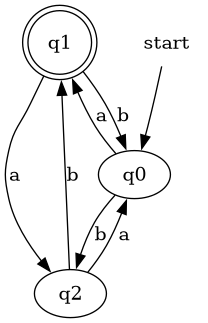
\includegraphics[width=0.4\textwidth]{buchi-automaton2.png} \\

\(A_4\):
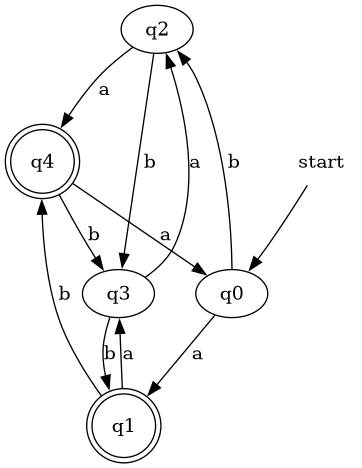
\includegraphics[width=0.4\textwidth]{buchi-automaton4.png} \\

Після виконання алгоритму композиції отримаємо наступні проміжні результати:

Двополюсник \(A_2\):
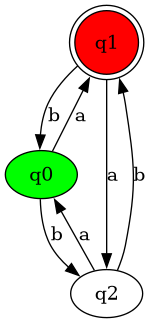
\includegraphics[width=0.3\textwidth]{bipole-automaton2.png} \\

Сильна ітерація \(A_4\):
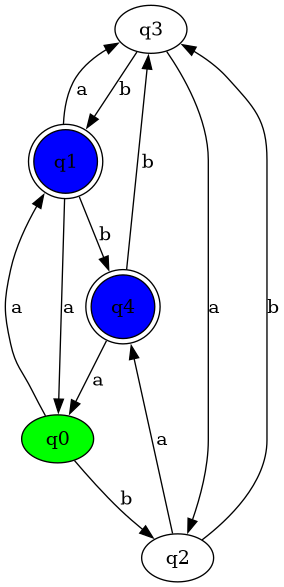
\includegraphics[width=0.3\textwidth]{strong-iteration-automaton4.png} \\

І нарешті, отримаємо складений автомат Бюхі \(B\) як результат композиції \(A_2\) та \(A_4\):

\(B\):
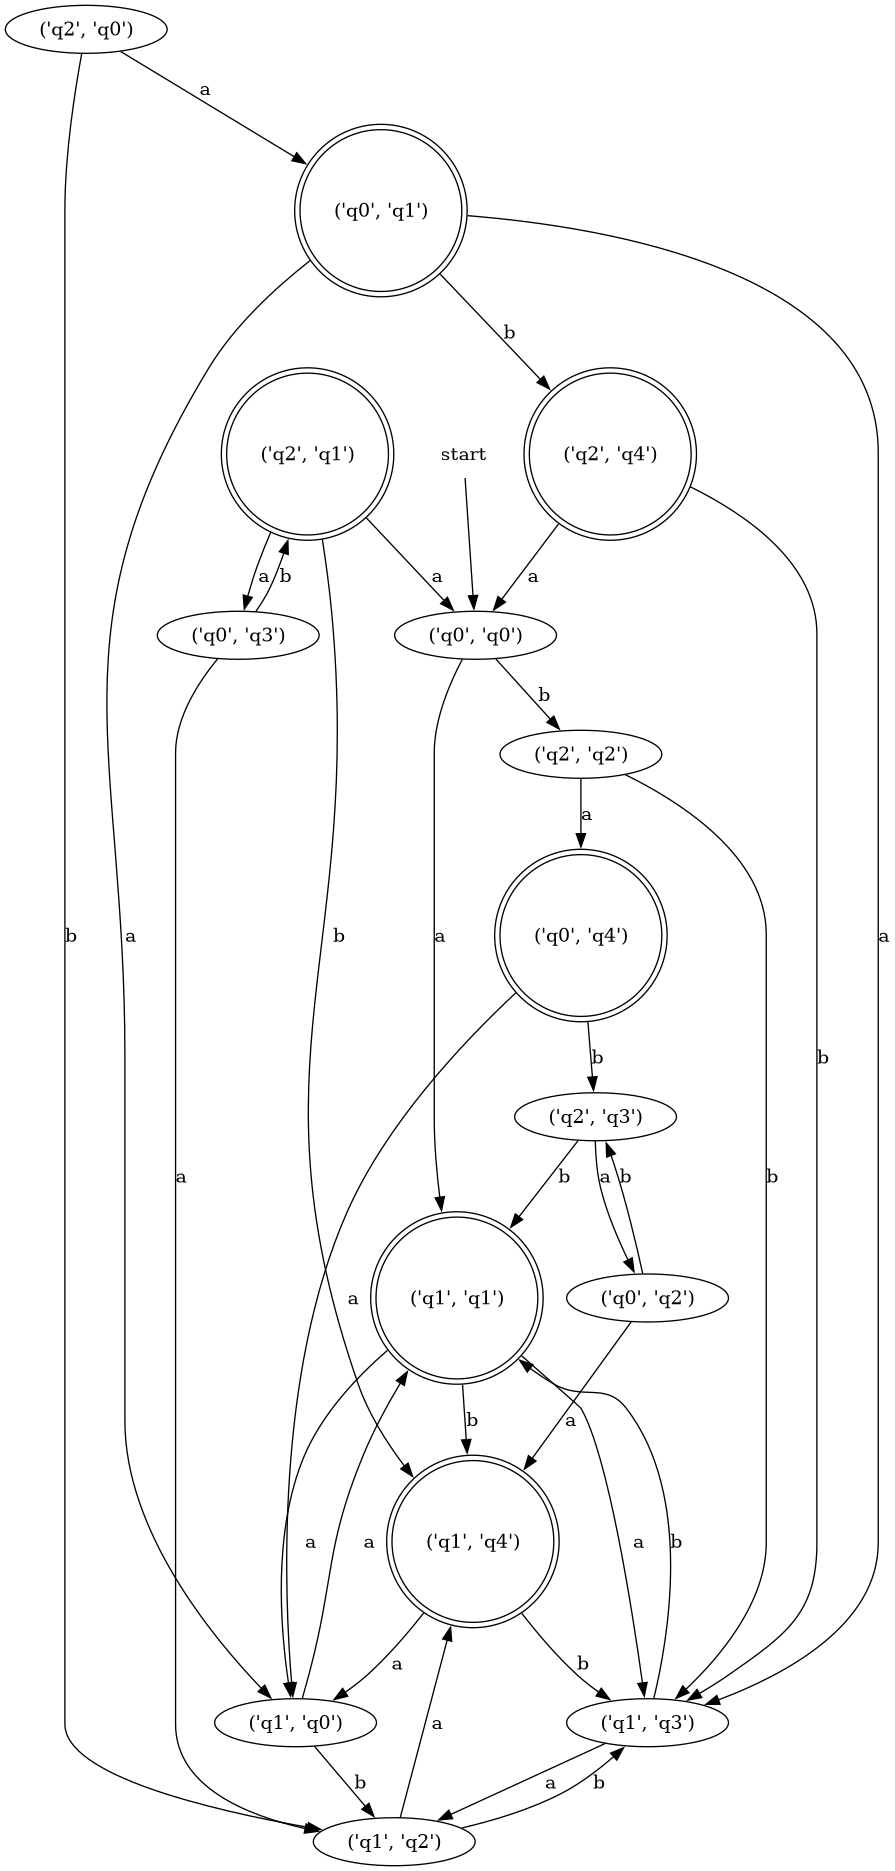
\includegraphics[width=0.4\textwidth]{concatenated-buchi-automaton2-automaton4.png} \\

Як видно, кожен перехід у результуючому автоматі Бюхі \(B\) є комбінацією переходів автоматів \(A_2\) та \(A_4\).

\newpage

\vspace{1em}
\textbf{Приклад 2:}
\vspace{0.5em}

Розглянемо два автомати Бюхі, \(A_3\) та \(A_6\), з наступними переходами:

\(A_3\):
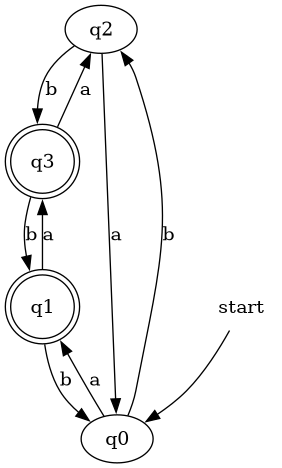
\includegraphics[width=0.4\textwidth]{buchi-automaton3.png} \\

\(A_6\):
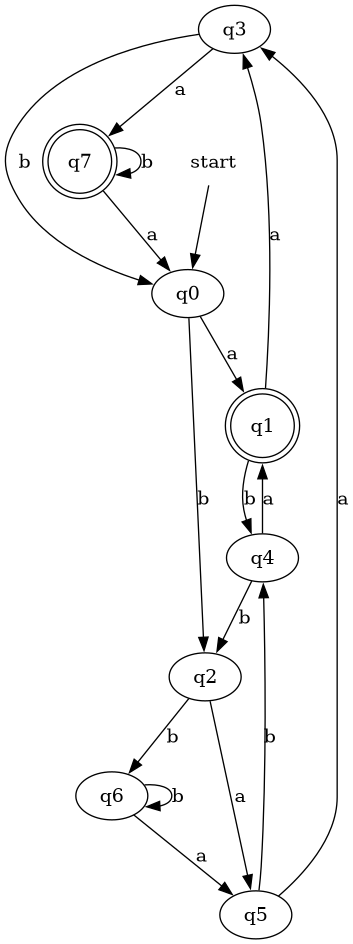
\includegraphics[width=0.4\textwidth]{buchi-automaton6.png} \\

Після виконання алгоритму композиції отримаємо наступні проміжні результати:

Двополюсник \(A_3\):
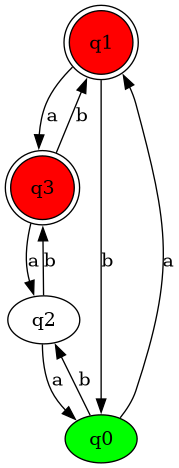
\includegraphics[width=0.3\textwidth]{bipole-automaton3.png} \\

Сильна ітерація \(A_6\):
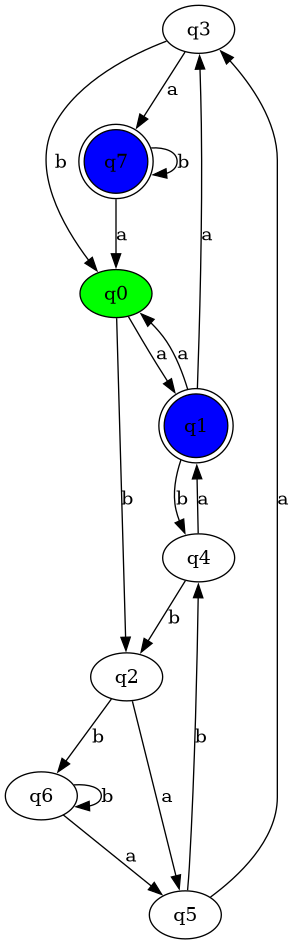
\includegraphics[width=0.3\textwidth]{strong-iteration-automaton6.png} \\

І нарешті, отримаємо складений автомат Бюхі \(B\) як результат композиції \(A_3\) та \(A_6\):

\(B\):
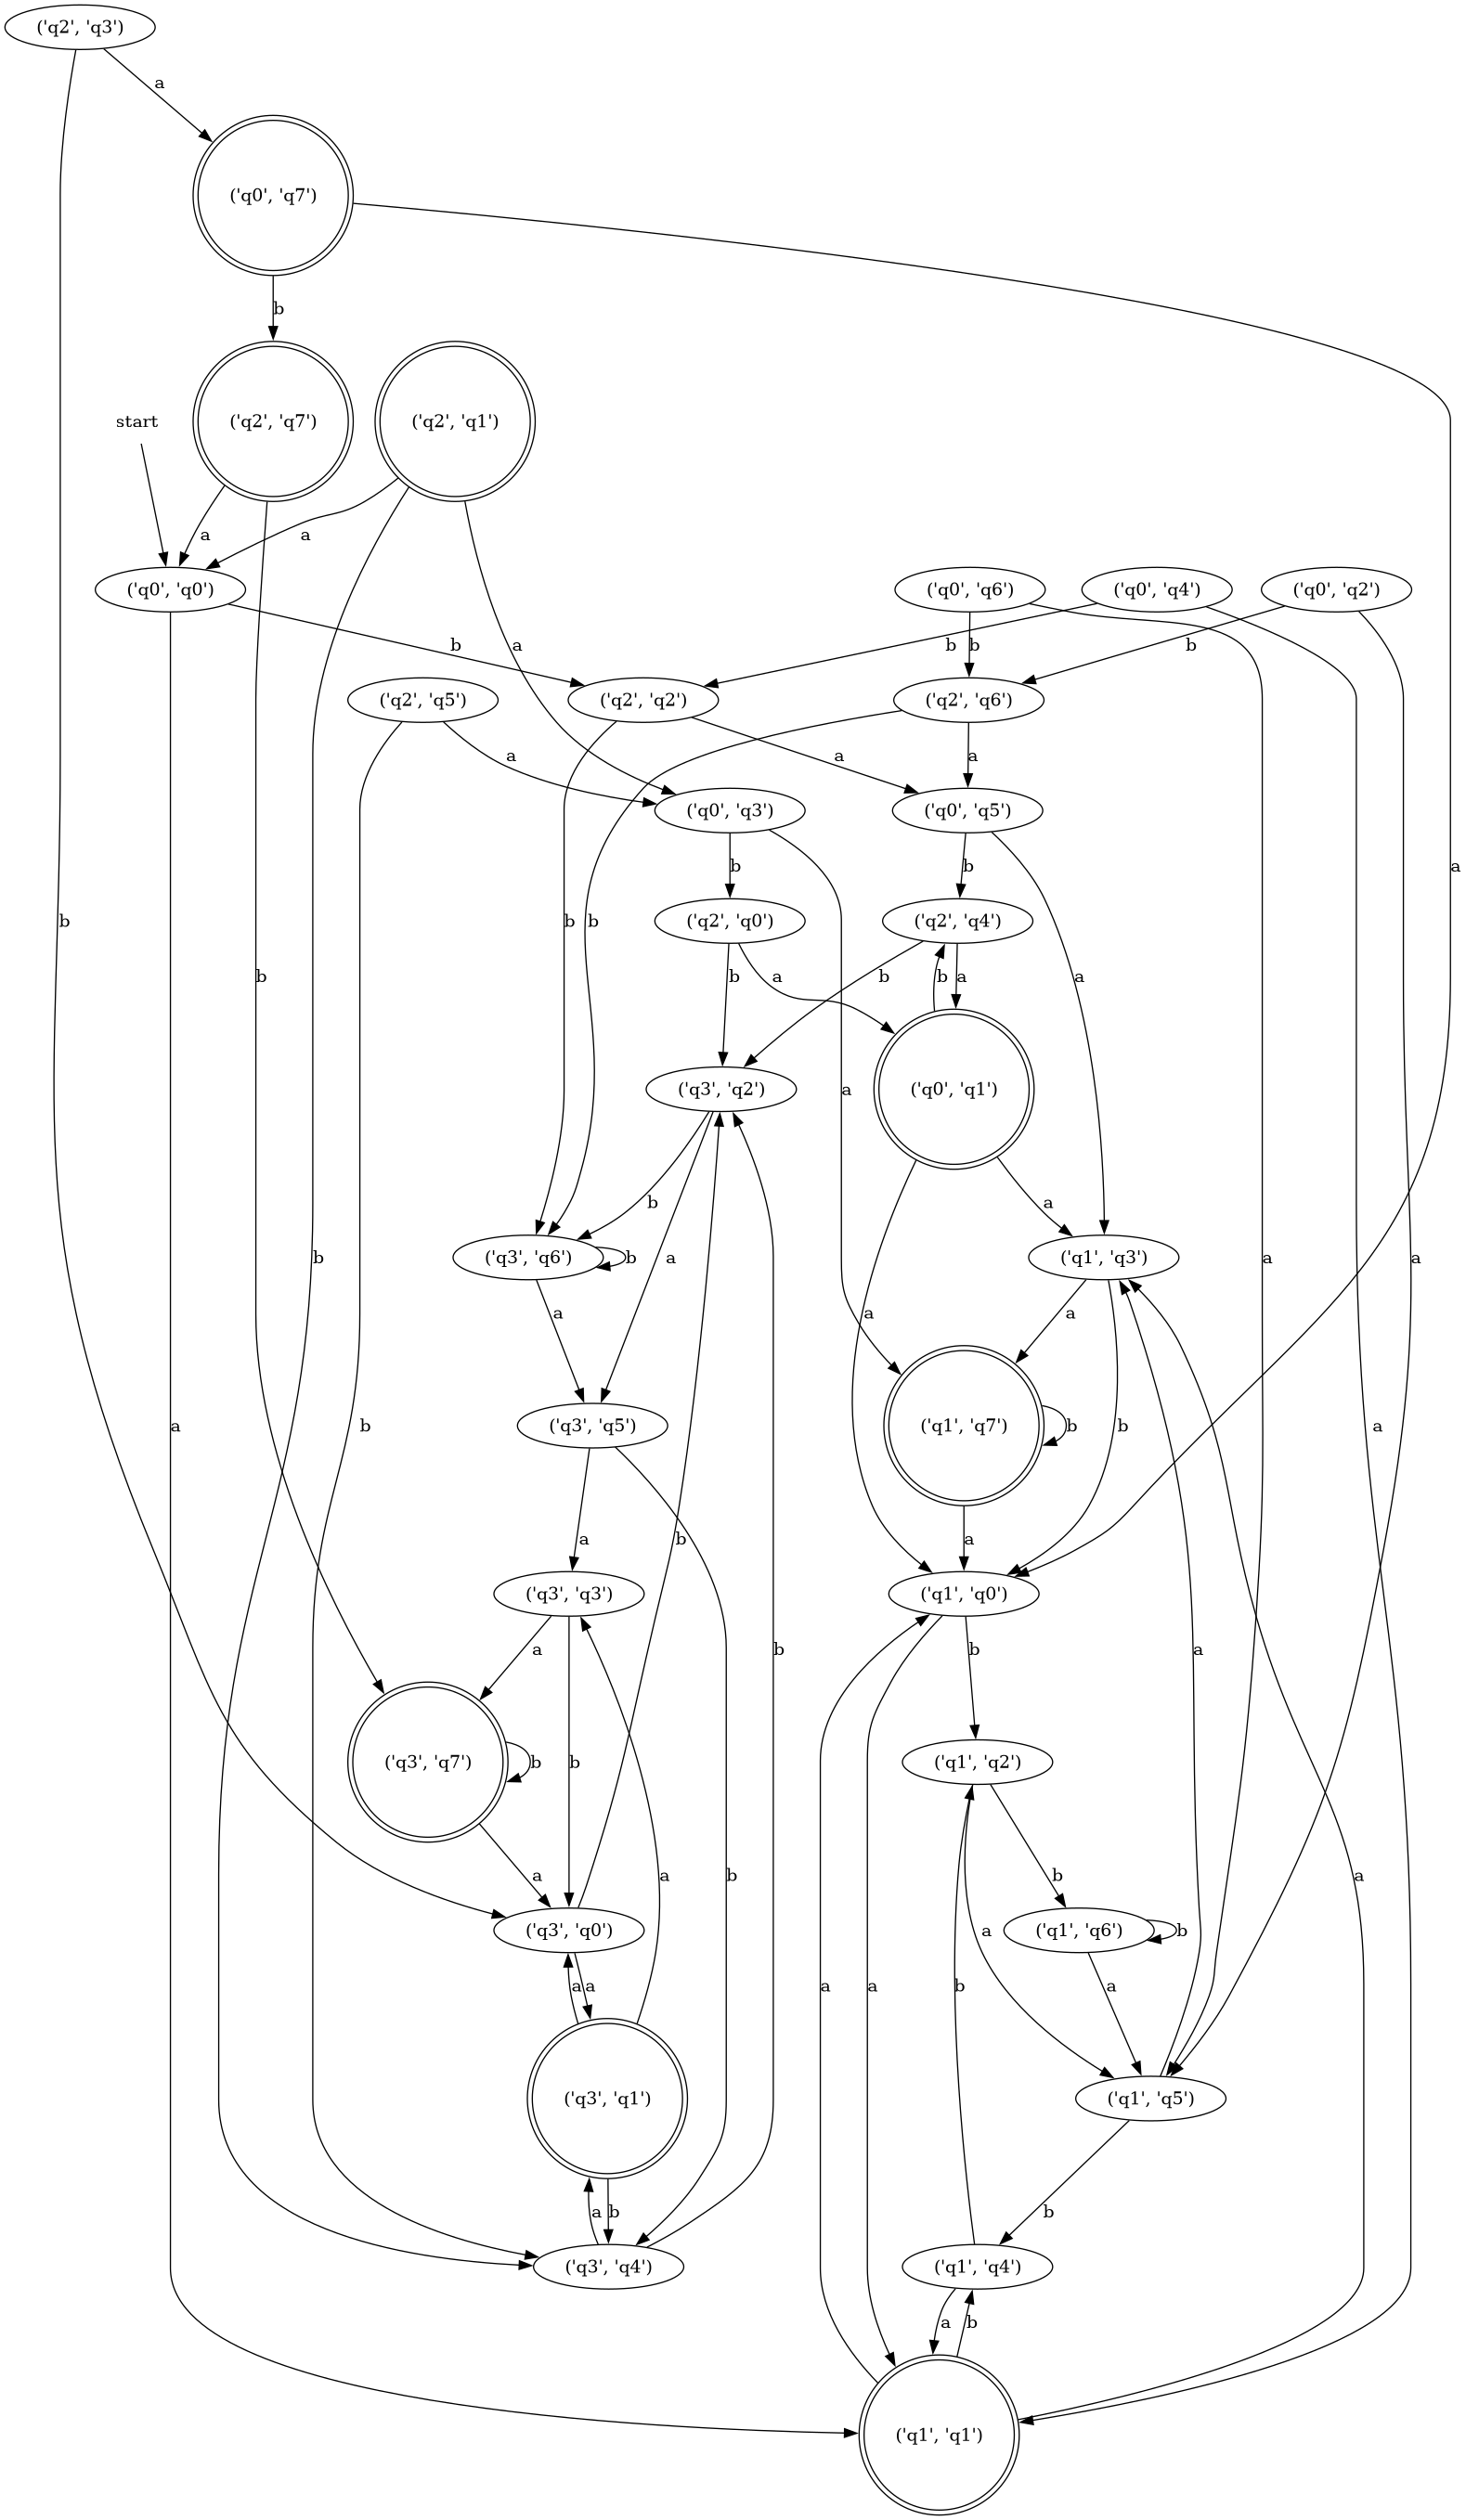
\includegraphics[width=0.4\textwidth]{concatenated-buchi-automaton3-automaton6.png} \\

Як видно, кожен перехід у результуючому автоматі Бюхі \(B\) є комбінацією переходів автоматів \(A_3\) та \(A_6\).

\newpage

\vspace{1em}
\textbf{Приклад 3:}
\vspace{0.5em}

Розглянемо два автомати Бюхі, \(A_4\) та \(A_1\), з наступними переходами:

\(A_4\):
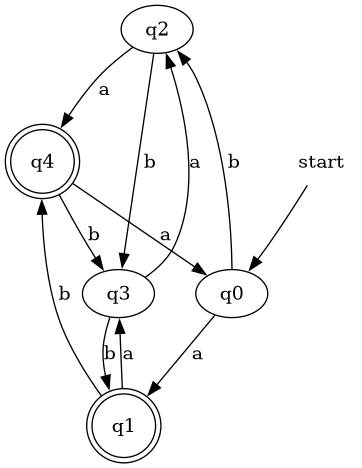
\includegraphics[width=0.4\textwidth]{buchi-automaton4.png} \\

\(A_1\):
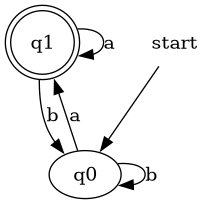
\includegraphics[width=0.4\textwidth]{buchi-automaton1.png} \\

Після виконання алгоритму композиції отримаємо наступні проміжні результати:

Двополюсник \(A_4\):
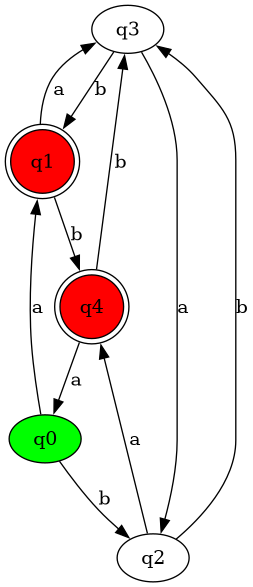
\includegraphics[width=0.3\textwidth]{bipole-automaton4.png} \\

Сильна ітерація \(A_1\):
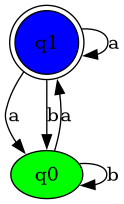
\includegraphics[width=0.3\textwidth]{strong-iteration-automaton1.png} \\

І нарешті, отримаємо складений автомат Бюхі \(B\) як результат композиції \(A_4\) та \(A_1\):

\(B\):
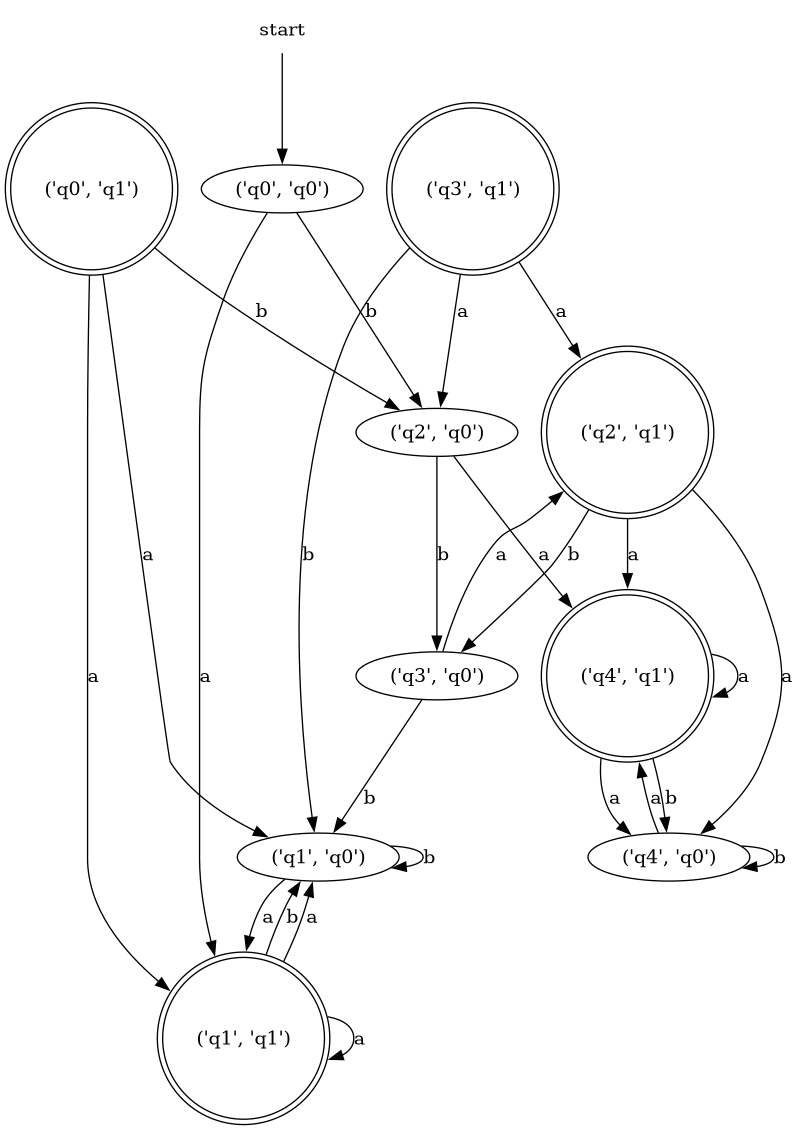
\includegraphics[width=0.4\textwidth]{concatenated-buchi-automaton4-automaton1.png} \\

Як видно, кожен перехід у результуючому автоматі Бюхі \(B\) є комбінацією переходів автоматів \(A_4\) та \(A_1\).

\newpage

\vspace{1em}
\textbf{Приклад 4:}
\vspace{0.5em}

Розглянемо два автомати Бюхі, \(A_5\) та \(A_3\), з наступними переходами:

\(A_5\):
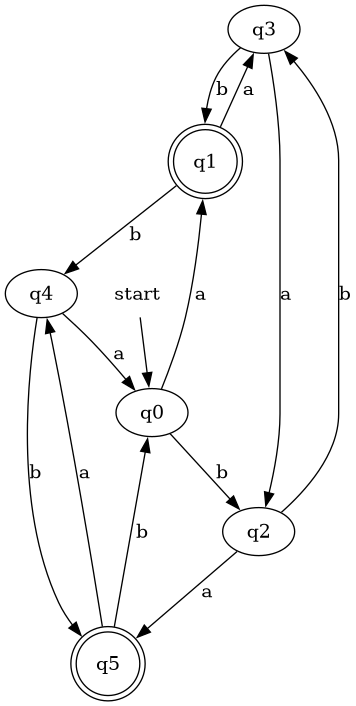
\includegraphics[width=0.4\textwidth]{buchi-automaton5.png} \\

\(A_3\):
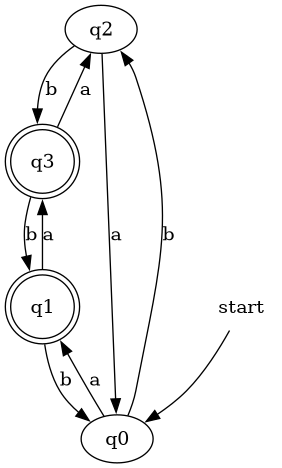
\includegraphics[width=0.4\textwidth]{buchi-automaton3.png} \\

Після виконання алгоритму композиції отримаємо наступні проміжні результати:

Двополюсник \(A_5\):
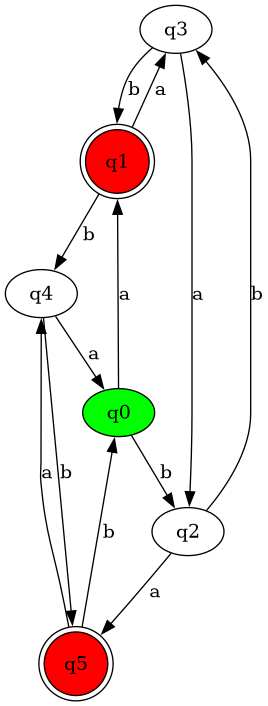
\includegraphics[width=0.3\textwidth]{bipole-automaton5.png} \\

Сильна ітерація \(A_3\):
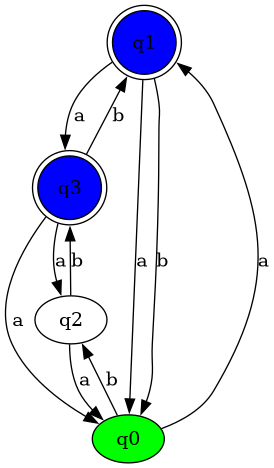
\includegraphics[width=0.3\textwidth]{strong-iteration-automaton3.png} \\

І нарешті, отримаємо складений автомат Бюхі \(B\) як результат композиції \(A_5\) та \(A_3\):

\(B\):
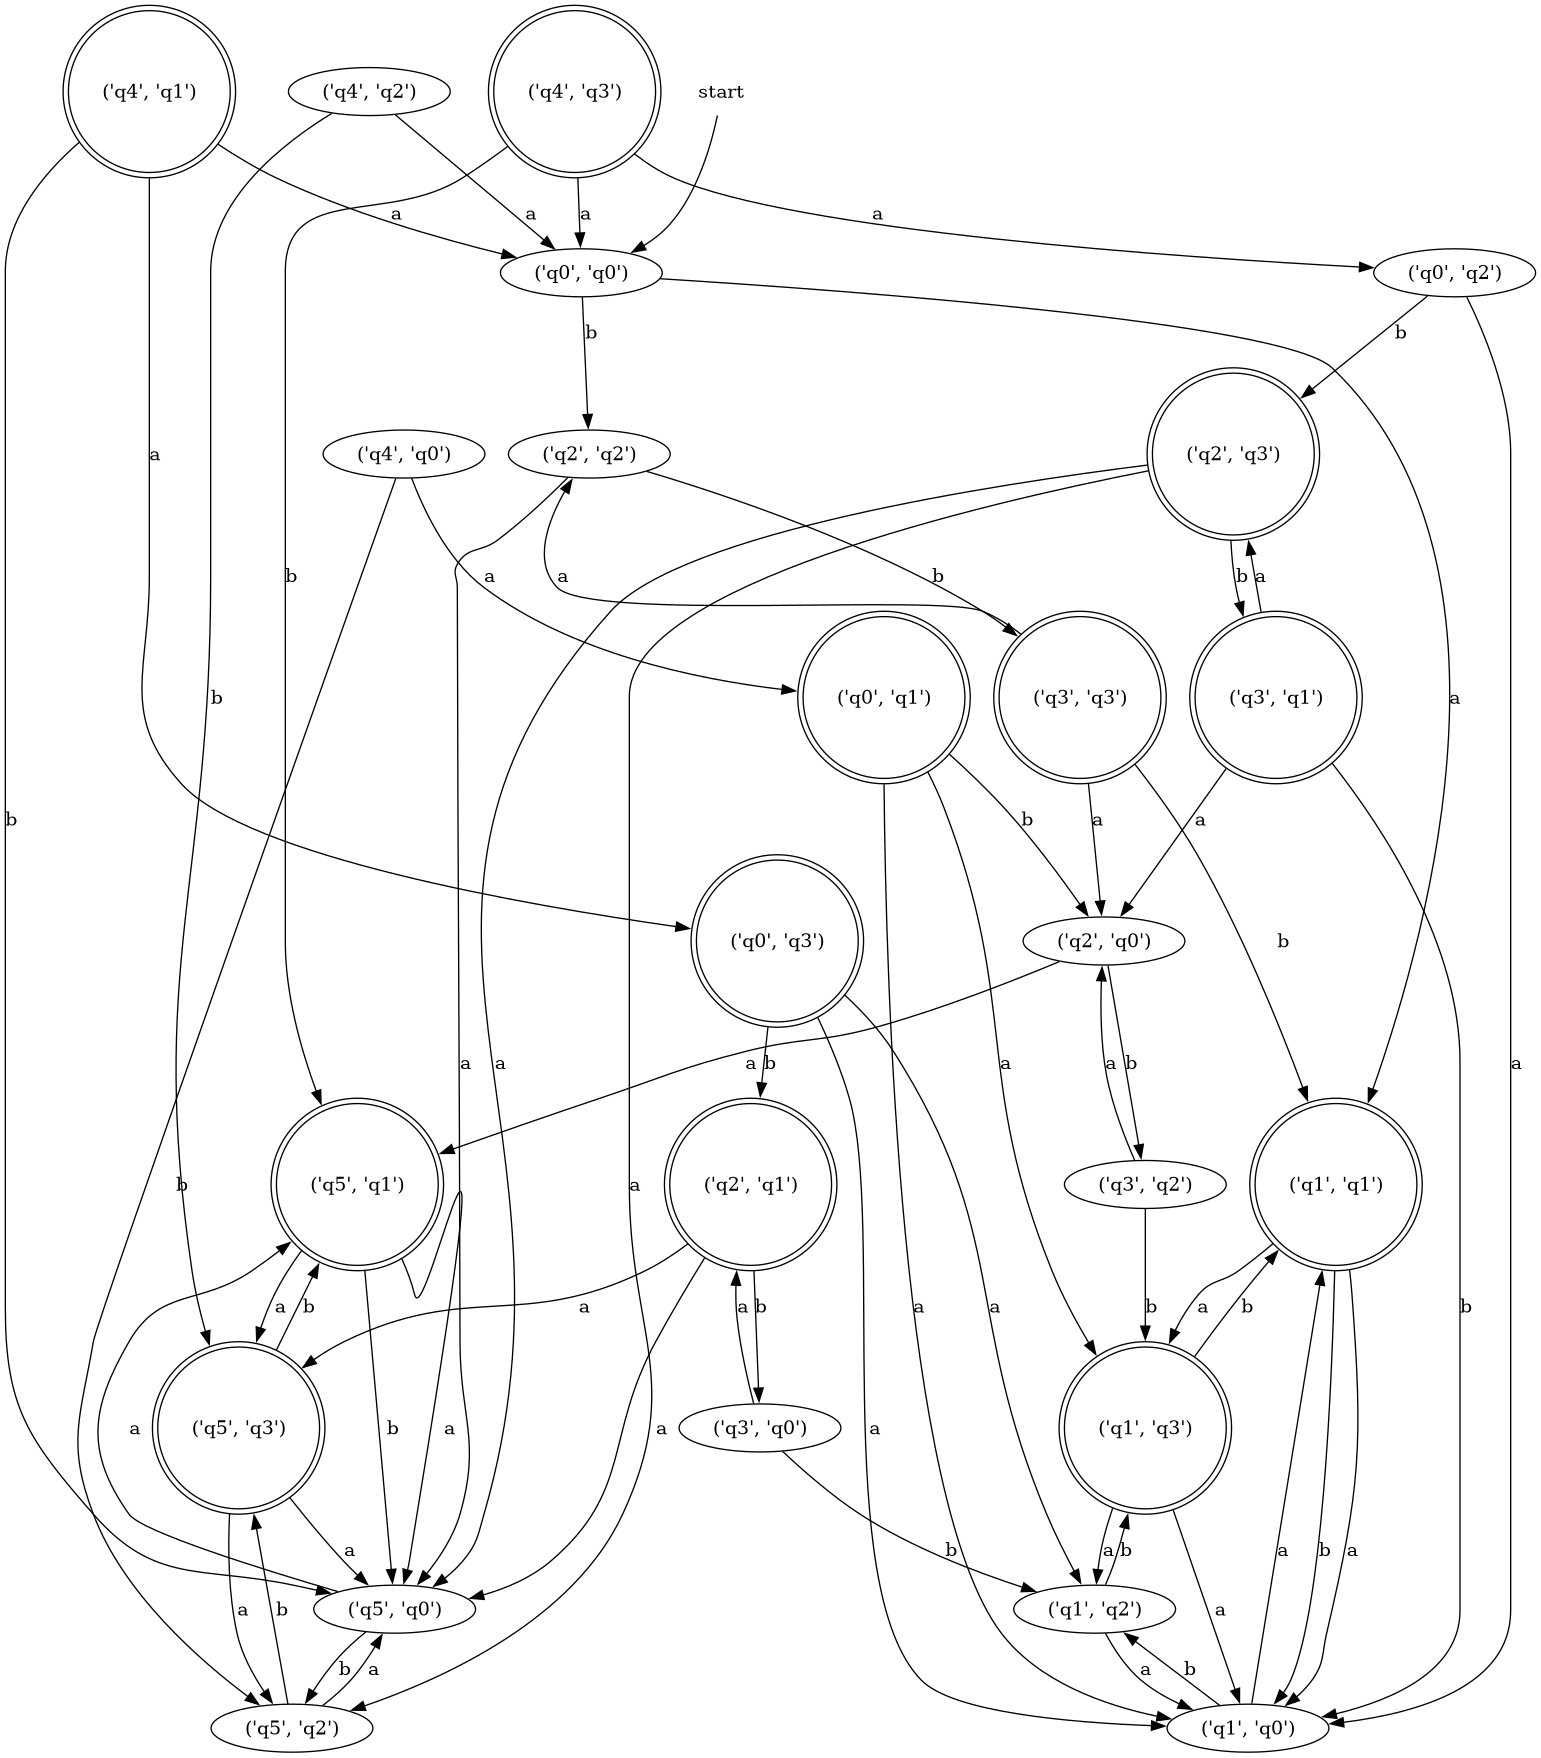
\includegraphics[width=0.4\textwidth]{concatenated-buchi-automaton5-automaton3.png} \\

Як видно, кожен перехід у результуючому автоматі Бюхі \(B\) є комбінацією переходів автоматів \(A_5\) та \(A_3\).

\newpage

\vspace{1em}
\textbf{Приклад 5:}
\vspace{0.5em}

Розглянемо два автомати Бюхі, \(A_6\) та \(A_2\), з наступними переходами:

\(A_6\):
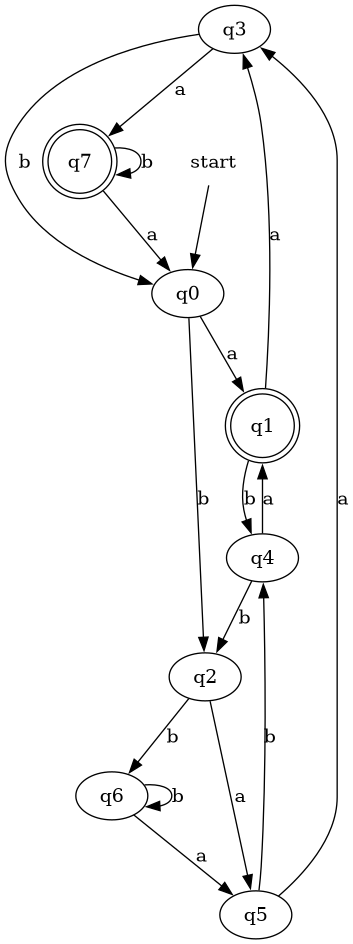
\includegraphics[width=0.4\textwidth]{buchi-automaton6.png} \\

\(A_2\):
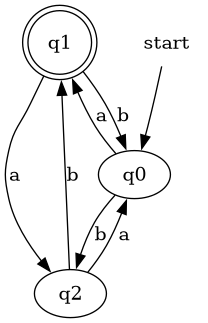
\includegraphics[width=0.4\textwidth]{buchi-automaton2.png} \\

Після виконання алгоритму композиції отримаємо наступні проміжні результати:

Двополюсник \(A_6\):
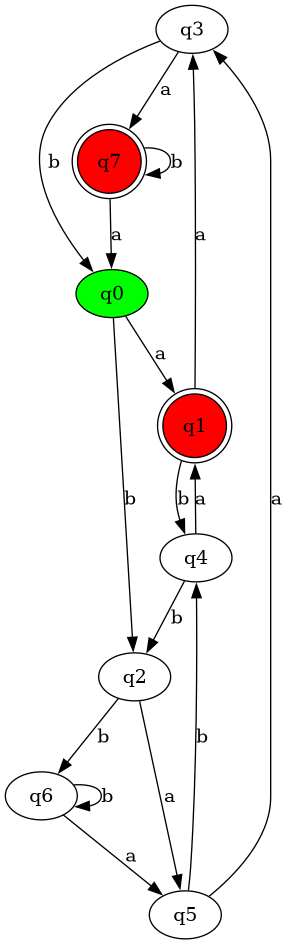
\includegraphics[width=0.3\textwidth]{bipole-automaton6.png} \\

Сильна ітерація \(A_2\):
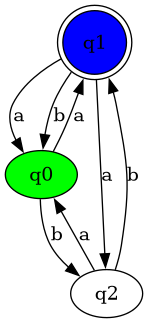
\includegraphics[width=0.3\textwidth]{strong-iteration-automaton2.png} \\

І нарешті, отримаємо складений автомат Бюхі \(B\) як результат композиції \(A_6\) та \(A_2\):

\(B\):
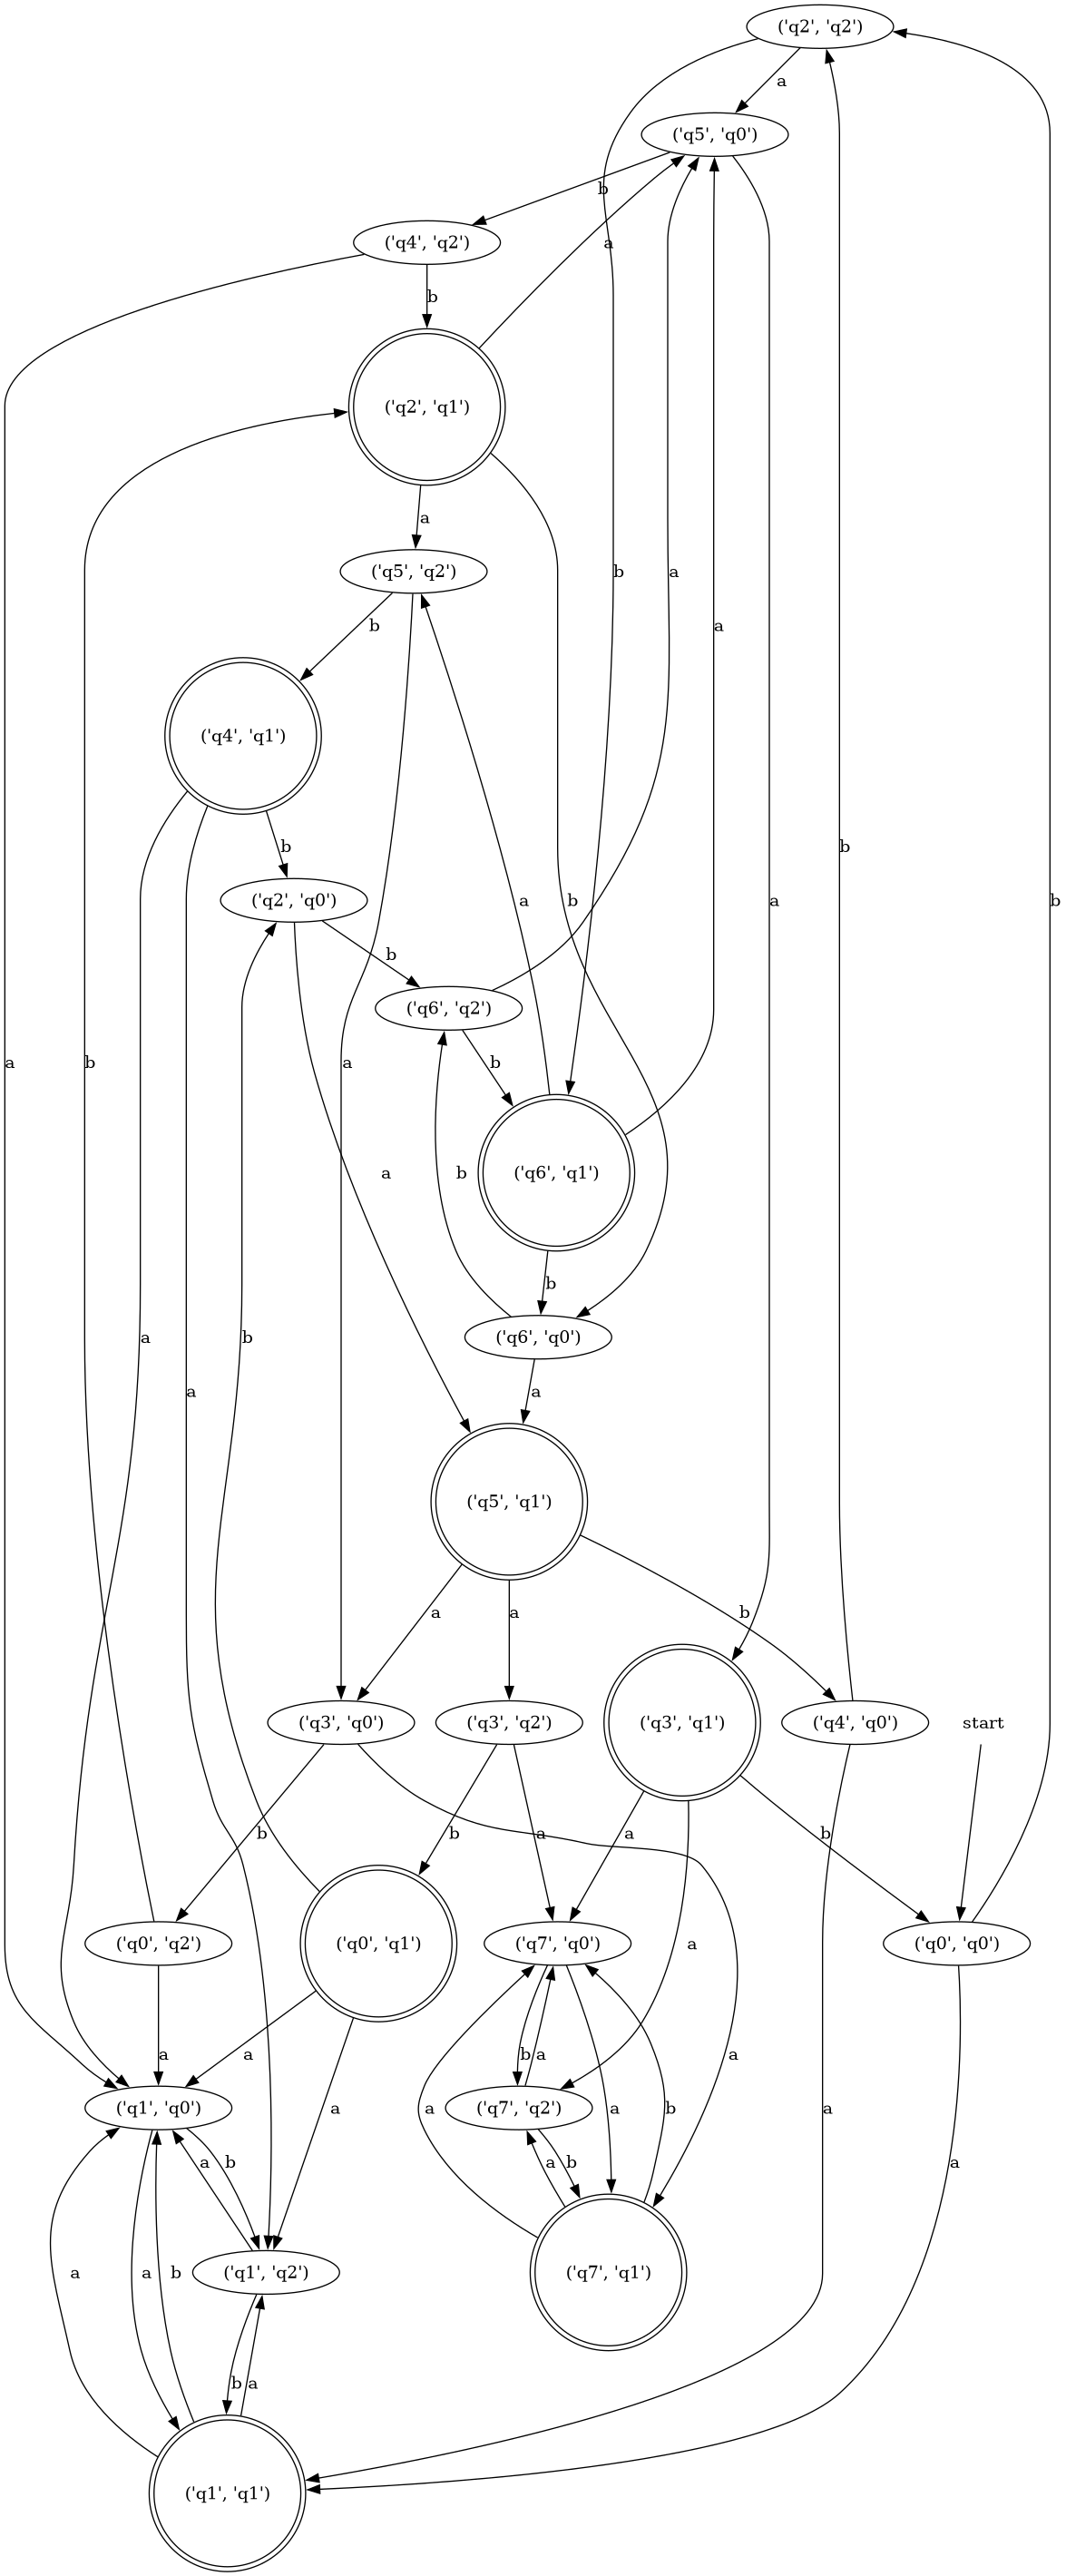
\includegraphics[width=0.4\textwidth]{concatenated-buchi-automaton6-automaton2.png} \\

Як видно, кожен перехід у результуючому автоматі Бюхі \(B\) є комбінацією переходів автоматів \(A_6\) та \(A_2\).

\newpage

\vspace{1em}
\textbf{Висновок:}
\vspace{0.5em}

У цьому звіті ми розглянули алгоритм для композиції двох Б'юхі автоматів та його практичне застосування на прикладах. Цей алгоритм є важливим інструментом у теорії автоматів, оскільки дозволяє поєднувати окремі автомати в один складний, здатний виконувати складніші завдання.

На прикладах, наведених у розділі \textref{sec:progress}{Хід роботи}, можна побачити, як алгоритм обробляє переходи вихідних автоматів та створює нові переходи для результуючих.

Таким чином, алгоритм композиції Б'юхі автоматів є потужним інструментом у теорії автоматів і може бути використаний для розширення можливостей автоматів та побудови більш складних систем.

\end{document}
